\documentclass[aspectratio=169,12pt]{beamer}
\usetheme{Madrid}
\usecolortheme{dolphin}
\usefonttheme{professionalfonts}
\setbeamertemplate{navigation symbols}{}
\setbeamertemplate{footline}{}

\usepackage[T1]{fontenc}
\usepackage[utf8]{inputenc}
\usepackage{graphicx}
\usepackage{amsmath,amssymb}
\usepackage{hyperref}
\usepackage{siunitx}
\usepackage{physics}

\begin{document}

\title[Chapter 2]{Chapitre 2: Vecteurs, qubit et superposition}
\author{JAMOTTE Maxime, SCHOONEN Cédric}
\institute{Digital Learning Hub}
\date{}

\begin{frame}
  \titlepage
\end{frame}

\begin{frame}
  \begin{enumerate}
    \item Vecteurs\\~\\
    \item Produit scalaire\\~\\
    \item Qubit, superposition d'états et vecteurs
  \end{enumerate}
\end{frame}

\begin{frame}{Vecteurs}
  {%
    \setbeamercolor{itemize/enumerate body}{fg=gray!60}
    \setbeamercolor{itemize item}{fg=gray!60}
    \setbeamercolor{alerted text}{fg=black}
    \begin{columns}[T]
      \begin{column}{0.55\textwidth}
        \begin{itemize}[<+-| alert@+>]
          \setlength{\itemsep}{0.6em}
          \item Définition d'un vecteur
          \item Addition de vecteurs
          \item Multiplication d'un vecteur par une constante
        \end{itemize}
        \bigskip
        \only<1>{\[
          \vec r = \begin{pmatrix} a \\ b \end{pmatrix}
        \]}
        \only<2>{\[
          \vec r + \vec p = 
          \begin{pmatrix} a \\ b \end{pmatrix} +
          \begin{pmatrix} c \\ d \end{pmatrix} =
          \begin{pmatrix} a+c \\ b+d \end{pmatrix}
        \]}
        \only<3>{\[
          \lambda \begin{pmatrix} a \\ b \end{pmatrix} =
          \begin{pmatrix} \lambda a \\ \lambda b \end{pmatrix}
        \]}
      \end{column}
      \begin{column}{0.4\textwidth}
        \centering
        \only<1>{\includegraphics[width=\linewidth]{figures/vecteur.png}}
        \only<2>{\includegraphics[width=\linewidth]{figures/add_vecteurs.png}}
        \only<3->{\includegraphics[width=\linewidth]{figures/multiplication_nombre.png}}
      \end{column}
    \end{columns}
  }
\end{frame}

\begin{frame}{Produit scalaire}
  \begin{itemize}[<+->]
    \setlength{\itemsep}{0.6em}
    \item La probabilité d'obtenir un résultat de mesure vient (en gros) d'une comparaison de deux états quantiques.
    \item Cette comparaison se traduit par un produit scalaire entre leurs vecteurs associés.
    $$\begin{pmatrix} a \\ b \end{pmatrix} \cdot \begin{pmatrix} c \\ d \end{pmatrix} = \begin{pmatrix} a & b \end{pmatrix} \begin{pmatrix} c \\ d \end{pmatrix} = ac+bd$$
  \end{itemize}
\end{frame}

\begin{frame}{Qubit}
  \begin{itemize}[<+->]
    \setlength{\itemsep}{0.6em}
    %\item Electron autour du noyau: infinité de positions possibles.
    \item L'électron passe à travers les fentes du haut ($H$) et du bas ($B$) en même temps.% $\ket{\psi_e^{}} = \alpha \ket{H} + \beta \ket{B}$.
      \only<1->{%
        \vspace{0.5em}
        \begin{center}
          \begin{minipage}{0.42\textwidth}
            \centering
            \includegraphics[width=0.6\linewidth]{figures/fente_Young.png}
          \end{minipage}\hfill
          \begin{minipage}{0.42\textwidth}
            \centering
            \only<2->{\includegraphics[width=0.6\linewidth]{figures/bohr_model.png}}
          \end{minipage}
        \end{center}
      }
    \item Certains systèmes physiques ont des niveaux discrets d'énergie (au lieu de la position).
    \item \textbf{Qubit} (= bit quantique) = système quantique à 2 niveaux, notés $\ket 0$ et $\ket 1$.
  \end{itemize}
\end{frame}

\begin{frame}{Superposition d'états et vecteurs}
  \begin{columns}[T]
    \begin{column}{0.6\textwidth}
      \begin{itemize}[<+->]
        \item Un qubit peut être dans $\ket 0$, $\ket 1$ ou toute \textbf{superposition} des deux: $\alpha \ket 0 + \beta \ket 1$.
        \item Superposition = combinaison linéaire d'états.
        \item \textbf{Postulat} : les états quantiques forment un espace vectoriel (espace de Hilbert). Une combinaison linéaire d'états est aussi un état.
        \item On note aussi $\ket 0 = \begin{pmatrix}1 \\ 0\end{pmatrix}$ et $\ket 1 = \begin{pmatrix}0 \\ 1\end{pmatrix}$.\\~\\
        \item État général : $\ket {\psi} = \alpha \ket 0 + \beta \ket 1$,\\~\\
        \item Une superposition $\alpha \ket 0 + \beta \ket 1$ s'écrit $\begin{pmatrix} \alpha \\ \beta \end{pmatrix}$.\\~\\
        %\item Probabilités de mesure : $P(\ket 0)=|\alpha|^2$, $P(\ket 1)=|\beta|^2$,
        %$$ \Longrightarrow  |\alpha|^2 + |\beta|^2 = 1$$
      \end{itemize}
    \end{column}
    \begin{column}{0.35\textwidth}
      \vspace{2em}
      \centering
      \only<4->{\includegraphics[width=0.8\textwidth]{figures/ket_base.png}}
    \end{column}
  \end{columns}
\end{frame}

\begin{frame}
  \centering
  Fin du chapitre 2: voyons comment manipuler les qubits!
\end{frame}

%##################
%##################

\title[Chapter 3]{Chapitre 3: Matrices, portes logiques classiques et quantiques}
\author{JAMOTTE Maxime, SCHOONEN Cédric}
\institute{Digital Learning Hub}
\date{}

\begin{frame}
  \titlepage
\end{frame}

\begin{frame}{Les matrices et leur action sur un vecteur}
  {%
    \setbeamercolor{itemize/enumerate body}{fg=gray!60}
    \setbeamercolor{itemize item}{fg=gray!60}
    \setbeamercolor{alerted text}{fg=black}
    \begin{columns}[T]
      \begin{column}{0.55\textwidth}
        \begin{itemize}[<+-| alert@+>]
          \setlength{\itemsep}{0.6em}
          \item Addition de matrices
          \item Multiplication d'une matrice par un scalaire
          \item Multiplication matrice-vecteur
        \end{itemize}
        \bigskip
        \only<1>{\[M_1^{}+M_2^{} = 
          \begin{pmatrix} a & b\\ c & d \end{pmatrix} +
          \begin{pmatrix} e & f\\ g & h \end{pmatrix} =
          \begin{pmatrix} a+e & b+f\\ c+g & d+h \end{pmatrix}
        \]}
        \only<2>{\[ \lambda M = 
          \lambda \begin{pmatrix} a & b\\ c & d \end{pmatrix} =
          \begin{pmatrix} \lambda a & \lambda b\\ \lambda c & \lambda d \end{pmatrix}
        \]}
        \only<3>{\[M \vec{r} = 
          \begin{pmatrix} a & b \\ c & d \end{pmatrix}
          \begin{pmatrix} u \\ v \end{pmatrix} =
          \begin{pmatrix} au + bv \\ cu + dv \end{pmatrix}
        \]}
      \end{column}
      \begin{column}{0.4\textwidth}
        \centering
        \only<1>{\fbox{\Large $M_1^{}+M_2^{}$}}
        \only<2>{\fbox{\Large $\lambda M$}}
        \only<3->{\includegraphics[width=\linewidth]{figures/multiplication_Mv.png}}
      \end{column}
    \end{columns}
  }
\end{frame}



\begin{frame}{Multiplication de deux matrices}

  \[ M_1^{} \times M_2^{} = \begin{pmatrix}
      a & b \\
      c & d
    \end{pmatrix}
    \begin{pmatrix}
      u_1^{} & u_2^{} \\
      v_1^{} & v_2^{}
    \end{pmatrix}
    =
    \begin{pmatrix}
      au_1^{} + bv_1^{} & au_2^{} + bv_2^{} \\
      cu_1^{} + dv_1^{} & cu_2^{} + dv_2^{}
    \end{pmatrix}
  \]
\\~\\
\end{frame}

\begin{frame}{Multiplication de matrices}

  \[ M_1^{} \times M_2^{} = \begin{pmatrix}
      a & b \\
      c & d
    \end{pmatrix}
    \begin{pmatrix}
      u_1^{} & u_2^{} \\
      v_1^{} & v_2^{}
    \end{pmatrix}
    =
    \begin{pmatrix}
      au_1^{} + bv_1^{} & au_2^{} + bv_2^{} \\
      cu_1^{} + dv_1^{} & cu_2^{} + dv_2^{}
    \end{pmatrix}
  \]
\\~\\
    \textbf{Non commutatif} en général : $M_1^{} \times M_2^{} \neq M_2^{} \times M_1^{}$.
  
  \bigskip
  \[
    \begin{pmatrix}
      0 & 1 \\
      1 & 0
    \end{pmatrix}
    \begin{pmatrix}
      1 & 0 \\
      0 & -1
    \end{pmatrix}
    =
    \begin{pmatrix}
      0 & -1 \\
      1 & 0
    \end{pmatrix}
      \]
  \bigskip
  \[
    \begin{pmatrix}
      1 & 0 \\
      0 & -1
    \end{pmatrix}
    \begin{pmatrix}
      0 & 1 \\
      1 & 0
    \end{pmatrix}
    =
    \begin{pmatrix}
      0 & 1 \\
      -1 & 0
    \end{pmatrix}
  \]
\end{frame}


\begin{frame}{Portes logiques classiques}
  \begin{itemize}[<+->]
    \setlength{\itemsep}{0.55em}
    \item Bits classiques: 0 ou 1; les portes transforment ces bits.
    \item Exemples clés : NOT, AND, OR, XOR, NAND (porte universelle).
    \item On enchaîne ces portes pour construire des circuits logiques.
  \end{itemize}
  \vfill
  \only<2->{%
    \centering
    \includegraphics[height=1.1cm]{figures/NOT.png}\hspace{0.3cm}
    \includegraphics[height=1.1cm]{figures/AND.png}\hspace{0.3cm}
    \includegraphics[height=1.1cm]{figures/OR.png}\hspace{0.3cm}
    \includegraphics[height=1.1cm]{figures/XOR.png}\hspace{0.3cm}
    \includegraphics[height=1.1cm]{figures/NAND.png}
  }
\end{frame}

\begin{frame}{Table de vérité (rappel)}
  \centering
  \begin{tabular}{l c c c}
    \textbf{Porte} & \textbf{Symbole} & \textbf{Expression} & \textbf{Description} \\\hline
    NOT   & $\lnot A$ & inverse & $1\leftrightarrow 0$ \\
    AND   & $A\cdot B$ & $1$ si $A=1$ et $B=1$ & porte "multiplication" \\
    OR    & $A + B$ & $1$ si $A=1$ ou $B=1$ & porte "addition" \\
    XOR   & $A \oplus B$ & $1$ si $A\neq B$ & "ou exclusif" \\
    NAND  & $\lnot(A\cdot B)$ & inverse de AND & base universelle \\
  \end{tabular}
\end{frame}

\begin{frame}{Table de vérité XOR / AND}
  \centering
  \begin{tabular}{c c | c | c}
    $A$ & $B$ & $A\ \mathbf{XOR}\ B$ & $A\ \mathbf{AND}\ B$ \\\hline
    0 & 0 & 0 & 0 \\
    0 & 1 & 1 & 0 \\
    1 & 0 & 1 & 0 \\
    1 & 1 & 0 & 1 \\
  \end{tabular}
\end{frame}

\begin{frame}{Exemple de circuit classique}
  \begin{itemize}[<+->]
    \item Enchaînement de portes pour additionner deux bits (avec report).
    \item Chaque fil transporte un bit, chaque symbole applique une porte.
  \end{itemize}
  \vfill
  \centering
  \includegraphics[width=0.65\textwidth]{figures/addition_circuit2.png}
\end{frame}

\begin{frame}{Portes logiques quantiques}
  \begin{itemize}[<+->]
    \setlength{\itemsep}{0.55em}
    \item Les qubits se transforment via des portes logiques quantiques.\\~\\
    \item Les \textbf{vecteurs} représentant les \textbf{qubits} sont transformés par des \textbf{matrices}
     représentant les \textbf{portes quantiques} (unitaires = ne changent pas la longueur du vecteur).\\~\\
    \item Exemples de portes: Pauli X (inversion), Z (phase), Hadamard $H$ (création de superposition).\\~\\
    \item Les circuits quantiques enchaînent ces portes sur des lignes de qubits (analogie classique).
  \end{itemize}
\end{frame}

\begin{frame}{Porte $X$ (NOT quantique)}
  \[
    X = \begin{pmatrix}0 & 1 \\ 1 & 0\end{pmatrix}
  \]
  ~\\~\\
  \[
    X\ket 0 = \ket 1, \qquad
    X\ket 1 = \ket 0
  \]
  ~\\~\\
  \[
    \begin{pmatrix}0 & 1 \\ 1 & 0\end{pmatrix}
    \begin{pmatrix}1\\0\end{pmatrix}=
    \begin{pmatrix}0\\1\end{pmatrix},
    \qquad
    \begin{pmatrix}0 & 1 \\ 1 & 0\end{pmatrix}
    \begin{pmatrix}0\\1\end{pmatrix}=
    \begin{pmatrix}1\\0\end{pmatrix}
  \]
\end{frame}

\begin{frame}{Porte $Z$ (phase)}
  \[
    Z = \begin{pmatrix}1 & 0 \\ 0 & -1\end{pmatrix}
  \]
  ~\\~\\
  \[
    Z\ket 0 = \ket 0, \qquad
    Z\ket 1 = -\ket 1
  \]
  ~\\~\\
  \[
    \begin{pmatrix}1 & 0 \\ 0 & -1\end{pmatrix}
    \begin{pmatrix}1\\0\end{pmatrix}=
    \begin{pmatrix}1\\0\end{pmatrix},
    \qquad
    \begin{pmatrix}1 & 0 \\ 0 & -1\end{pmatrix}
    \begin{pmatrix}0\\1\end{pmatrix}=
    \begin{pmatrix}0\\-1\end{pmatrix}
  \]
\end{frame}

\begin{frame}{Porte $H$ (Hadamard)}
  \[
    H = \tfrac{1}{\sqrt{2}}\begin{pmatrix}1 & 1 \\ 1 & -1\end{pmatrix}
  \]
  ~\\~\\
  \[
    H\ket 0 = \tfrac{1}{\sqrt{2}}(\ket 0+\ket 1), \qquad
    H\ket 1 = \tfrac{1}{\sqrt{2}}(\ket 0-\ket 1)
  \]
  ~\\~\\
  \[
    \tfrac{1}{\sqrt{2}}\begin{pmatrix}1 & 1 \\ 1 & -1\end{pmatrix}
    \begin{pmatrix}1\\0\end{pmatrix}=
    \tfrac{1}{\sqrt{2}}\begin{pmatrix}1\\1\end{pmatrix},
    \qquad
    \tfrac{1}{\sqrt{2}}\begin{pmatrix}1 & 1 \\ 1 & -1\end{pmatrix}
    \begin{pmatrix}0\\1\end{pmatrix}=
    \tfrac{1}{\sqrt{2}}\begin{pmatrix}1\\-1\end{pmatrix}
  \]
\end{frame}

% \begin{frame}{Mesure d'un qubit}
%   \begin{itemize}[<+->]
%     \setlength{\itemsep}{0.55em}
%     \item Mesurer projette l'état sur $\ket 0$ ou $\ket 1$.
%     \item Probabilités : $P(\ket 0)=|\alpha|^2$, $P(\ket 1)=|\beta|^2$ pour $\alpha\ket 0+\beta\ket 1$.
%     \item L'état post-mesure est figé sur le résultat observé (effondrement).
%   \end{itemize}
% \end{frame}

\begin{frame}[plain]
  \centering
  \vfill
  {\Large Fin du chapitre 3: passons à la pratique avec QISKIT!}
  \vfill
\end{frame}

\end{document}
